% 第4章
%!TEX root = main.tex
本章では,に示した数理計画モデルによる,
実際の水系に準ずる例題を用いた計算例を示し,%
構築したモデルの妥当性について検討する.
なお,求解には数理計画パッケージCPLEX12\cite{cplex}を用いた.
%%%%%%%%%%
\section{問題設定}
%%%%%%%%%%

計画期間を24時間,時間帯幅を10分とした問題を考える.
Fig. \ref{fig:watersystem}およびFig. \ref{fig:value}に対象とする水系と%
各時間帯における発電価値を示す.
発電価値は需要が多い時間帯に高くなることから,%
今回は需要曲線を元に作成したものを使用した.
Fig. \ref{fig:watersystem}における,台形,長方形および円形のシンボルがそれぞれダム,%
分流施設,発電放流路を表している.\\
また,Tables. \ref{storage}〜\ref{storage2}に水系の基本情報などのパラメータの設定値を示す.
\indent
問題の設定として,以下を想定する.
\begin{itemize}
	\item
	スイッチ放流路$\rm Y_{5,6},\rm Y_{5,7}$は%
	発電機$\rm G_{810}$系と対応しており,$\rm G_{810}$系の運転時には$\rm Y_{5,7}$に%
	放流を行ない,停止時には$\rm Y_{5,6}$に放流を行なう.
	\item
	目的関数については$w=100,000$とし,ゲート放流に対するペナルティが%
	大きくなるようにすることで,ゲート放流量を可能な限り抑える.
	\item
	短時間運転・停止制約における連続運転・停止期間を%
	1時間として設定する.
	\item
	20時から6時を夜間とする.
	\item
	計画運転・停止期間は設定しない.
	\item
	$\rm D_{2}$については,そこからの発電放流量は%
	すべて予め計画されているものとする.
	\item
	バイパス放流量および渓流量はそれぞれの放流路やダムで常に一定とし,
	1時間帯当たりの水量をTable. \ref{bypass}および\ref{stream}に示す.
\end{itemize}

\begin{figure}[H]
  \centering
  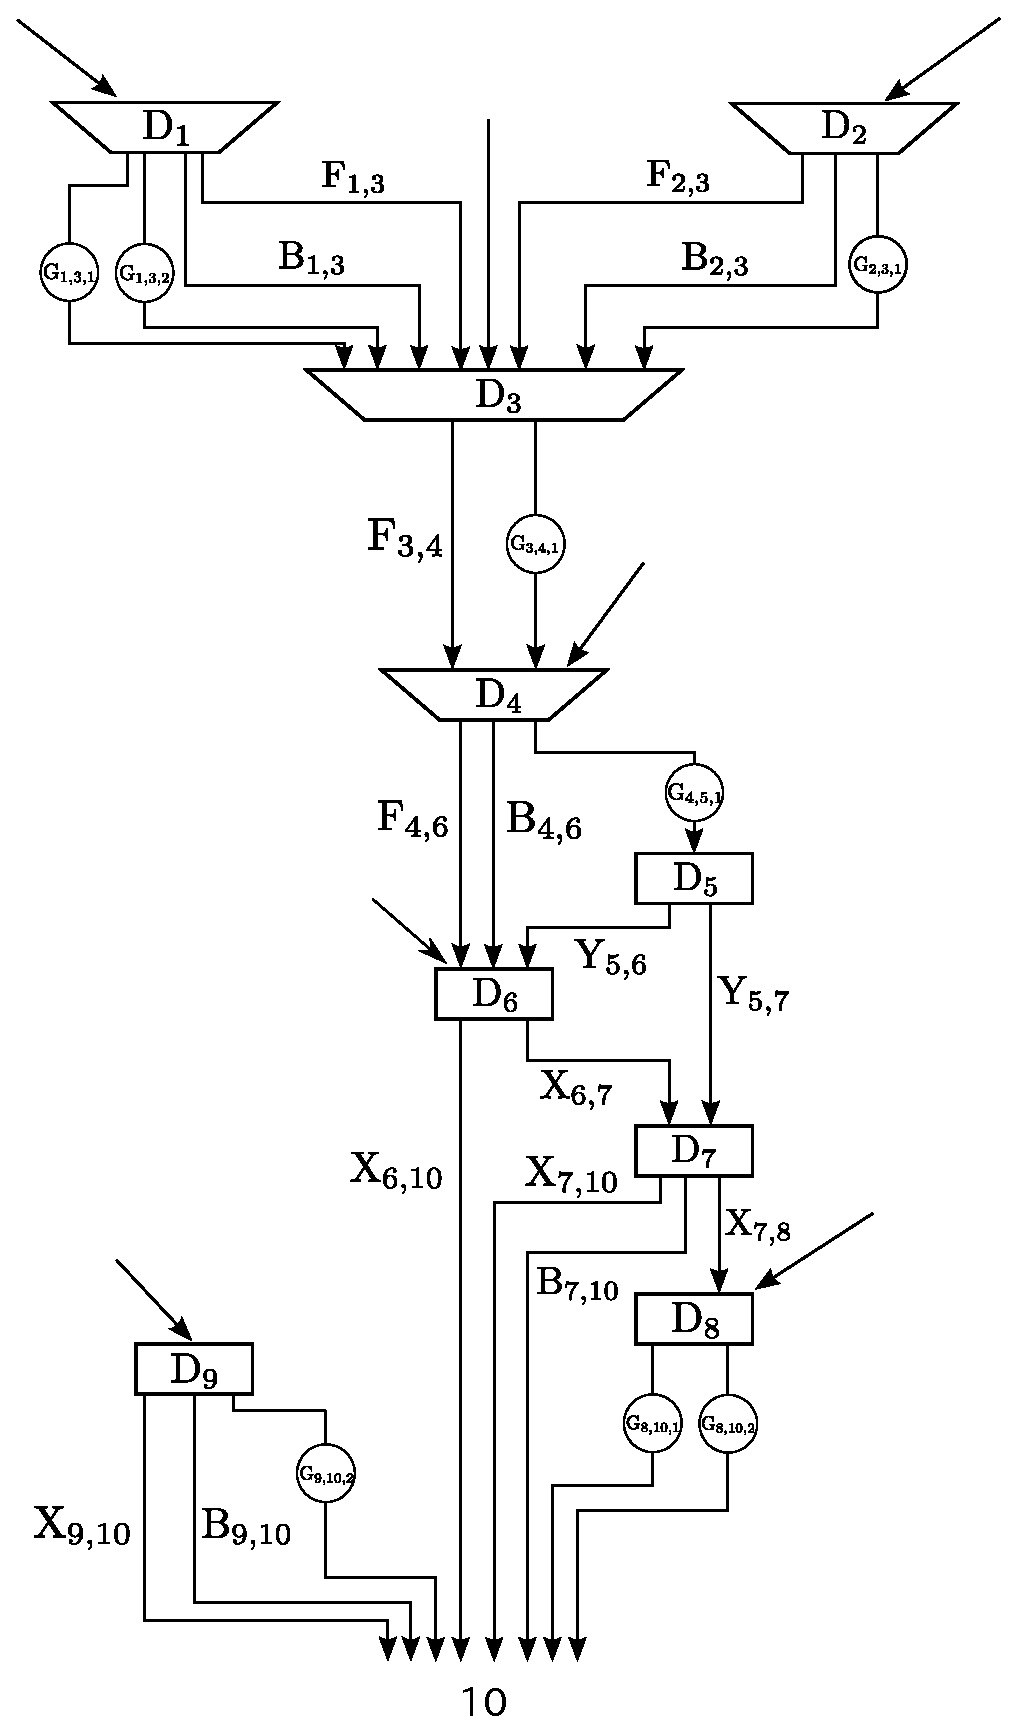
\includegraphics[width=0.85\linewidth]{fig/JinzuRev3.eps}
  \caption{Water system}
  \label{fig:watersystem}
\end{figure}

\begin{figure}[H]
  \centering
  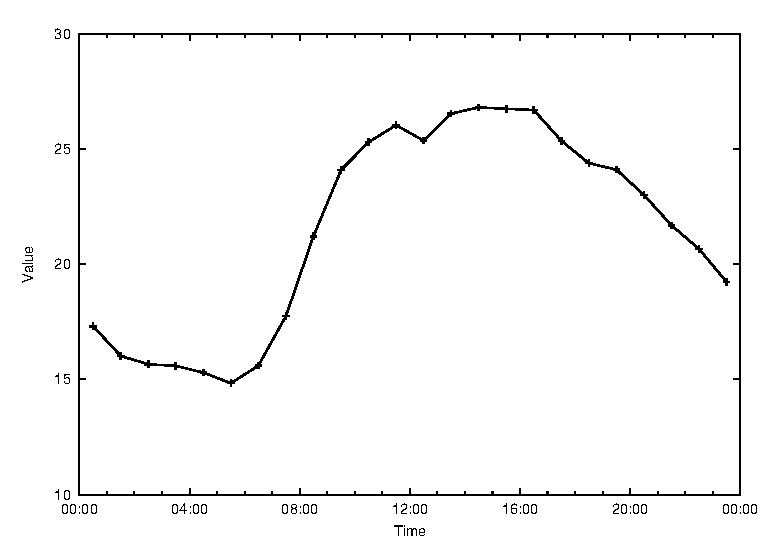
\includegraphics[width=0.9\linewidth]{fig/val.eps}
  \caption{Value of electric energy}
  \label{fig:value}
\end{figure}

\begin{table}[htbp]
\begin{center}
\caption{Storage of dam}
\label{storage}
\begin{tabular}{llllll}
\hline
Number & 1 & 2 & 3 & 4\\
\hline \hline
$s^{\rm Min}$ & 142,707 & 0 & 625,409 & 1,152,112 & \\
$s^{\rm Max}$ & 553,791 & 117,935,420 & 1,370,298 & 2,698,099\\
\hline
\end{tabular}
\label{storage}
\end{center}
\end{table}

\begin{table}[htbp]
\label{table:7}
\begin{center}
\caption{Generator Data}
\vspace*{-5mm}
\begin{tabular}{ccccccccc}
\hline
Generator Number & 131 & 132 & 231 & 341 & 451 & 8101 & 8102 & 9101 \\ \hline \hline
$q^{\rm G,Max}$[$\rm{m^3}$] & 20640 & 20640 & 39000 & 22200 & 23640 & 13080 & 13080 & 3000 \\
$q^{\rm G,Min}$[$\rm{m^3}$] & 5400 & 5400 & 8520 & 7041 & 8006 & 1344 & 1344 & 124\\
$\alpha$[$\rm{kWh/m^3}$] & 0.0788 & 0.0786 & 0.6069 & 0.0583 & 0.1680 & 0.3250 & 0.3222 & 0.6888\\
$\tau^{\rm G,Up}$ & 0 & 0 & 0 & 0 & 0 & 0 & 0  & 0 \\
$\tau^{\rm G,Down}$ & 2 & 2 & 1 & 2 & 2 & 0 & 0  & 0 \\
\hline
\end{tabular}
\end{center}
\end{table}

\begin{table}[htbp]
\begin{center}
\caption{Gate waterway Data}
\label{gate}
\begin{tabular}{ccccccc}
\hline
Number &13 & 23 & 34 & 46 \\ \hline \hline
$q^{\rm F,Max}$[$\rm {10^{-4} \cdot m^3}$] & 138 & 102 & 174 & 180 \\
$\tau^{\rm F}$ & 0 & 0 & 0 & 0 \\
\hline
\end{tabular}
\end{center}
\end{table}

\begin{table}[htbp]
\begin{center}
\caption{Special waterway Data}
\label{way}
\begin{tabular}{llllll}
\hline
Number & 67 & 78 & 710 & 610 & 910\\ \hline
$q^{\rm X,Max}$[$ \rm {m^3}$] & 24,000 & 24,000 & 24,000 & 2,100,000 & 300,000 \\
$\tau^{\rm X}$& 0 & 0 & 0 & 0 & 0 \\
\hline
\end{tabular}
\end{center}
\end{table}

\begin{table}[htbp]
\begin{center}
\caption{Switch waterway Data}
\label{switch}
\label{table:way2}
\begin{tabular}{ccc}
\hline
Number & 56 & 57 \\ \hline
$q^{\rm Y,Max}$[$ \rm {m^3}$] & 23,700 & 23,700 \\
\hline
\end{tabular}
\end{center}
\end{table}

\begin{table}[htbp]
\begin{center}
\caption{First and last storage of dam}
\label{storage2}
\begin{tabular}{llllll}
\hline
Number & 1 & 2 & 3 & 4\\
\hline \hline
$s^{\rm Last,Min}$ & 409,419 & 26,340,350 & 1,156,164 & 2,247,878\\
first & 409,419 & 73,786,986 & 1,156,164 & 2,247,878 \\
$s^{\rm Last,Max}$ & 409,419 & 117,935,420 & 1,156,164 & 2,247,878\\
\hline
\end{tabular}
\label{storage}
\end{center}
\end{table}

\begin{table}[htbp]
\begin{center}
\caption{Bypass discharge}
\label{bypass}
\begin{tabular}{ccccc}
\hline
$\rm B_{13}$ & $\rm B_{23}$ & $\rm B_{46}$ & $\rm B_{710}$ & $\rm B_{910}$ \\
\hline
\hline
0 & 360 & 0 & 3,339 & 0\\
\hline
\end{tabular}
\end{center}
\end{table}

\begin{table}[htbp]
\begin{center}
\caption{Mountain stream}
\label{stream}
\begin{tabular}{ccccccccc}
\hline
1 & 2 & 3 & 4 & 5 & 6 & 7 & 8 & 9\\
\hline
\hline
3,000 & 3,000 & 1,200 & 3,000 & 0 & 0 & 0 & 0 & 1,440\\
\hline
\end{tabular}
\end{center}
\end{table}


\newpage
%%%%%%%%%%%%%%%%
\section{計算結果および考察}
%%%%%%%%%%%%%%%%

%目的関数値:47689359
%計算時間:31.95[sec]

Figs. \ref{fig:d1}〜\ref{fig:d9}に,結果として得られた各ダムの貯水量の推移と
そのダムからの発電放流量を示す%
(Figs. \ref{fig:d1}〜\ref{fig:d4}においては上下限貯水量も示している).
ただし,$\rm D_{8}$および$\rm D_{9}$は分流施設であり,貯水機能を持たないので,%
$\rm G_{8,10,1}$,$\rm G_{8,10,2}$,$\rm G_{9,10,1}$への%
発電放流量のみFig. \ref{fig:d8}およびFig. \ref{fig:d9}に示している.

Figs. \ref{fig:d1}〜\ref{fig:d8}の結果より,いずれの発電放流路においても,%
発電価値の高い時間帯での可能な限りの放流が行なわれる結果となっていることが
確認できる($\rm D_{9}$は渓流のみが流れ込む分流施設であるため,%
常に一定の発電放流を行なっている(Fig. \ref{fig:d9})).
また,貯水量および放流量の上下限等の制約も満たされていることがわかる.
これらより,本研究で構成した数理計画モデルは妥当なものであると考えられる.

\begin{figure}[H]
  \centering
  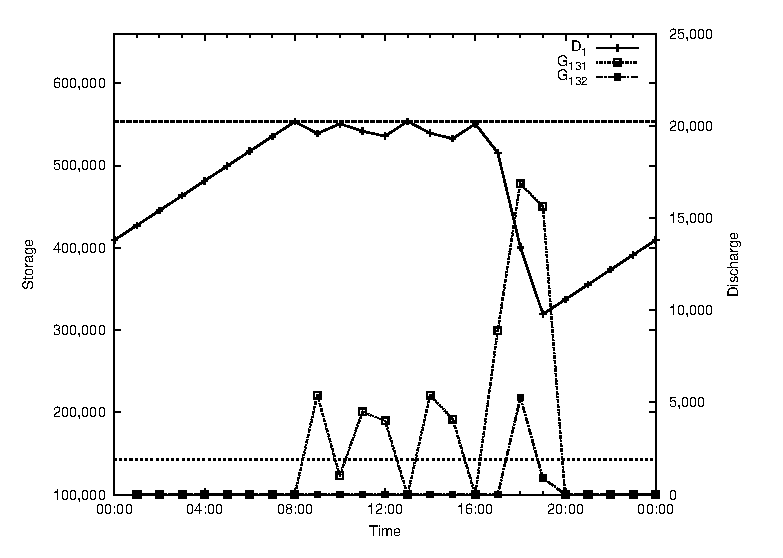
\includegraphics[width=0.9\linewidth]{fig/d1.eps}
  \caption{Storage in $\rm D_{1}$ and Generation Discharge}
  \label{fig:d1}
\end{figure}

\begin{figure}[H]
  \centering
  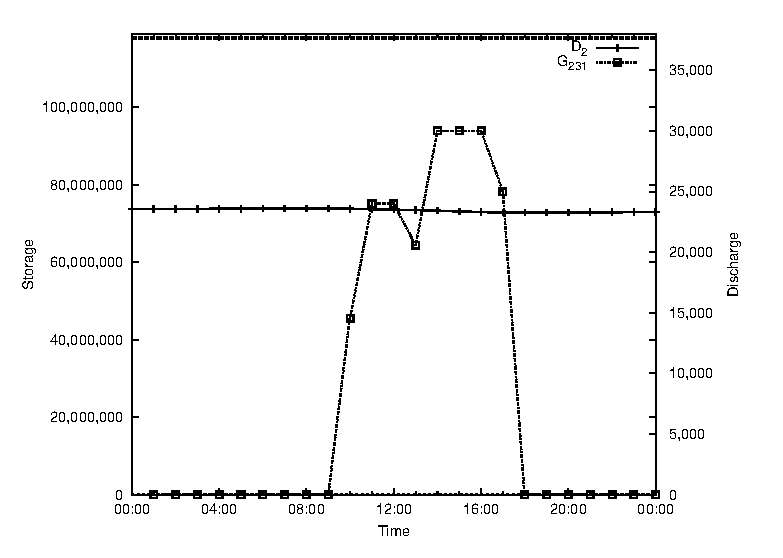
\includegraphics[width=0.9\linewidth]{fig/d2.eps}
  \caption{Storage in $\rm D_{2}$ and Generation Discharge }
  \label{fig:d2}
\end{figure}

\begin{figure}[H]
  \centering
  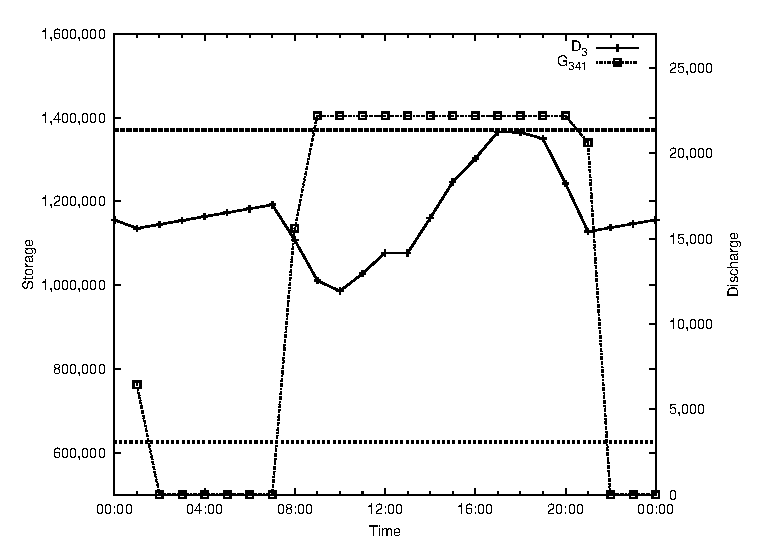
\includegraphics[width=0.9\linewidth]{fig/d3.eps}
  \caption{Storage in $\rm D_{3}$ and Generation Discharge }
  \label{fig:d3}
\end{figure}

\begin{figure}[H]
  \centering
  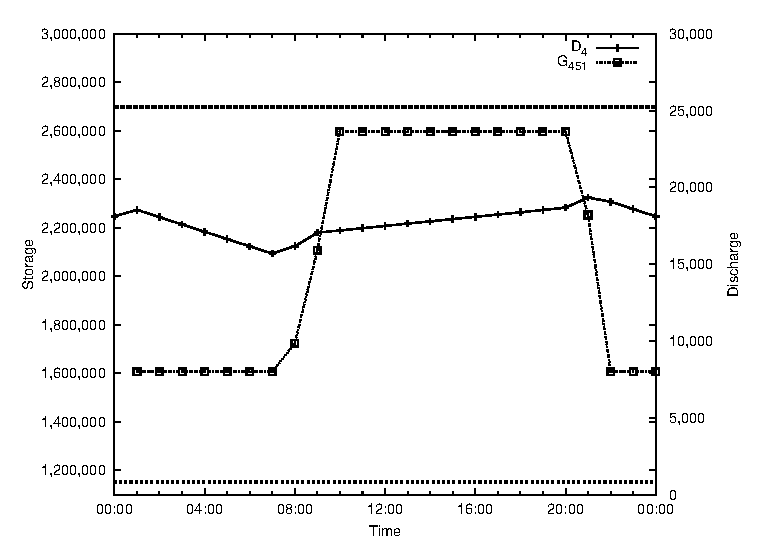
\includegraphics[width=0.9\linewidth]{fig/d4.eps}
  \caption{Storage in $\rm D_{4}$ and Generation Discharge }
  \label{fig:d4}
\end{figure}

\begin{figure}[H]
  \centering
  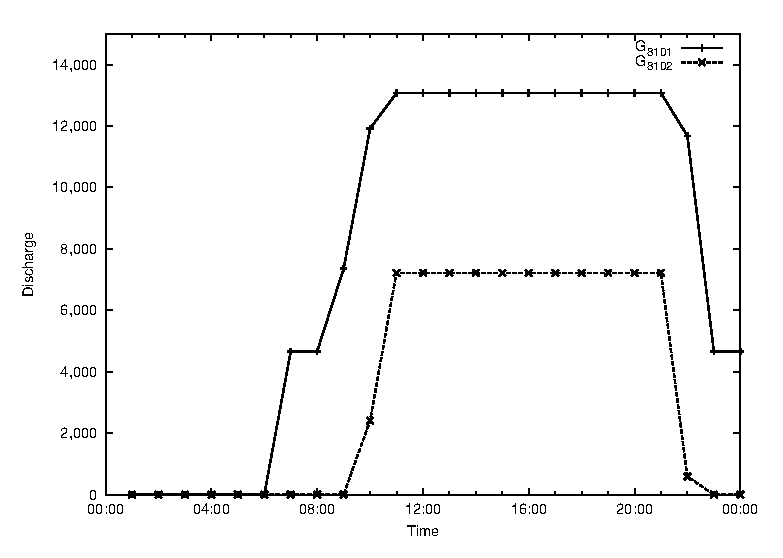
\includegraphics[width=0.9\linewidth]{fig/d8.eps}
  \caption{Discharge from $\rm D_{8}$}
  \label{fig:d8}
\end{figure}

\begin{figure}[H]
  \centering
  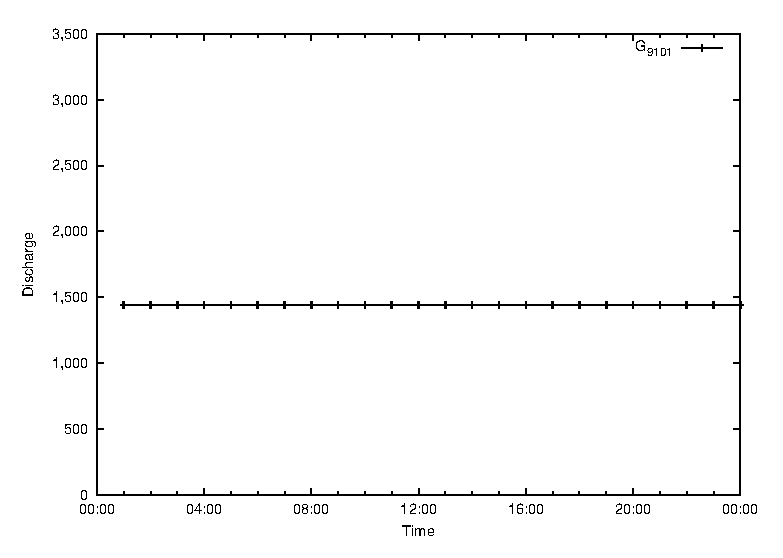
\includegraphics[width=0.9\linewidth]{fig/d9.eps}
  \caption{Discharge from $\rm D_{9}$}
  \label{fig:d9}
\end{figure}

%%%%%%%%%
\section{まとめ}
%%%%%%%%%

本章では,実際の水系に準ずる例題を用いた計算例を示し,%
その結果から提案モデルの妥当性を確認した.
次章では,結論として本研究で得られた成果と今後の課題を要約する.

